% ==========================================================================
% INFO 4617 Web Data Science -- Week 5: Web Architecture & Protocols (Chapter 5)
% Build:  TEXINPUTS=../common: BIBINPUTS=../common: latexmk -pdf slides.tex
% (or run `make` from the slides/ directory)
% ==========================================================================
\documentclass[9pt,aspectratio=169]{beamer}
% Resolve the shared theme/preamble in ../common/ when compiling this
% file directly from its own folder (no TEXINPUTS needed).
\makeatletter\def\input@path{{../common/}}\makeatother
% ==========================================================================
% Shared preamble for INFO 4617 Web Data Science weekly lecture decks
% Based on the Gotham beamer theme (vendored in this directory).
% Each week's slides.tex does:  % ==========================================================================
% Shared preamble for INFO 4617 Web Data Science weekly lecture decks
% Based on the Gotham beamer theme (vendored in this directory).
% Each week's slides.tex does:  % ==========================================================================
% Shared preamble for INFO 4617 Web Data Science weekly lecture decks
% Based on the Gotham beamer theme (vendored in this directory).
% Each week's slides.tex does:  \input{preamble}  (with common/ on TEXINPUTS)
% then sets \title/\subtitle/\author/\date and \begin{document}.
% ==========================================================================

\usetheme{gotham}

\usepackage{fbb}
\usepackage{booktabs}
\usepackage{graphicx}
\usepackage{tikz}
\usepackage{xcolor}
\usepackage{multirow}
\usepackage{listings}
\usetikzlibrary{positioning, arrows.meta, shapes}

% Bibliography
\usepackage[style=authoryear,
            backend=biber,
            maxcitenames=1,
            uniquename=false,
            uniquelist=false]{biblatex}
\addbibresource{bibliography.bib}

\gothamset{sectiontocframe default=off}

% ------------------------------------------------------------------ colors
\definecolor{cugold}{HTML}{CFB87C}
\definecolor{tab-red}{HTML}{E15759}
\definecolor{tab-orange}{HTML}{F28E2B}
\definecolor{tab-blue}{HTML}{4E79A7}
\definecolor{tab-cyan}{HTML}{76B7B2}
\definecolor{tab-green}{HTML}{59A14F}
\definecolor{tab-yellow}{HTML}{EDC948}
\definecolor{tab-purple}{HTML}{B07AA1}
\definecolor{tab-pink}{HTML}{FF9DA7}
\definecolor{tab-brown}{HTML}{9C755F}
\definecolor{tab-gray}{HTML}{BAB0AC}

\setbeamercolor{frametitle}{fg=black, bg=cugold}
\setbeamercolor{progress bar}{fg=cugold, bg=cugold!20}

\setbeamercolor{block title alerted}{fg=black, bg=cugold}
\setbeamercolor{block body alerted}{fg=black, bg=cugold!10}

% ------------------------------------------------------------------ footline
\setbeamertemplate{footline}{
  \begin{beamercolorbox}[wd=\paperwidth,ht=2.5ex,dp=1ex,right]{footline}
    {\footnotesize \insertframenumber{} of \inserttotalframenumber}
    \hspace*{2ex}
  \end{beamercolorbox}
}

% ------------------------------------------------------------------ helpers
\newcommand{\bottomcite}[1]{
    \vspace*{\fill}
    \vspace{-\baselineskip}
    {\tiny
    \rule{\textwidth}{0.3pt}\\
    #1
    }
    \vspace{0.5ex}
}

% Consistent code styling for the Wednesday "applied notebook" frames.
\lstdefinestyle{wds}{
    basicstyle=\ttfamily\scriptsize,
    keywordstyle=\color{tab-blue}\bfseries,
    commentstyle=\color{tab-green},
    stringstyle=\color{tab-orange},
    showstringspaces=false,
    breaklines=true,
    columns=fullflexible,
    language=Python,
    aboveskip=0.4em,
    belowskip=0.4em,
}
\lstset{style=wds}

% \dayband{Day}{Topic} -- a lightweight section divider label used to mark
% Monday / Wednesday / Friday within a week's deck.
\newcommand{\dayband}[2]{{\large\textbf{#1}}\;\textcolor{tab-gray}{\textbar}\;#2}
  (with common/ on TEXINPUTS)
% then sets \title/\subtitle/\author/\date and \begin{document}.
% ==========================================================================

\usetheme{gotham}

\usepackage{fbb}
\usepackage{booktabs}
\usepackage{graphicx}
\usepackage{tikz}
\usepackage{xcolor}
\usepackage{multirow}
\usepackage{listings}
\usetikzlibrary{positioning, arrows.meta, shapes}

% Bibliography
\usepackage[style=authoryear,
            backend=biber,
            maxcitenames=1,
            uniquename=false,
            uniquelist=false]{biblatex}
\addbibresource{bibliography.bib}

\gothamset{sectiontocframe default=off}

% ------------------------------------------------------------------ colors
\definecolor{cugold}{HTML}{CFB87C}
\definecolor{tab-red}{HTML}{E15759}
\definecolor{tab-orange}{HTML}{F28E2B}
\definecolor{tab-blue}{HTML}{4E79A7}
\definecolor{tab-cyan}{HTML}{76B7B2}
\definecolor{tab-green}{HTML}{59A14F}
\definecolor{tab-yellow}{HTML}{EDC948}
\definecolor{tab-purple}{HTML}{B07AA1}
\definecolor{tab-pink}{HTML}{FF9DA7}
\definecolor{tab-brown}{HTML}{9C755F}
\definecolor{tab-gray}{HTML}{BAB0AC}

\setbeamercolor{frametitle}{fg=black, bg=cugold}
\setbeamercolor{progress bar}{fg=cugold, bg=cugold!20}

\setbeamercolor{block title alerted}{fg=black, bg=cugold}
\setbeamercolor{block body alerted}{fg=black, bg=cugold!10}

% ------------------------------------------------------------------ footline
\setbeamertemplate{footline}{
  \begin{beamercolorbox}[wd=\paperwidth,ht=2.5ex,dp=1ex,right]{footline}
    {\footnotesize \insertframenumber{} of \inserttotalframenumber}
    \hspace*{2ex}
  \end{beamercolorbox}
}

% ------------------------------------------------------------------ helpers
\newcommand{\bottomcite}[1]{
    \vspace*{\fill}
    \vspace{-\baselineskip}
    {\tiny
    \rule{\textwidth}{0.3pt}\\
    #1
    }
    \vspace{0.5ex}
}

% Consistent code styling for the Wednesday "applied notebook" frames.
\lstdefinestyle{wds}{
    basicstyle=\ttfamily\scriptsize,
    keywordstyle=\color{tab-blue}\bfseries,
    commentstyle=\color{tab-green},
    stringstyle=\color{tab-orange},
    showstringspaces=false,
    breaklines=true,
    columns=fullflexible,
    language=Python,
    aboveskip=0.4em,
    belowskip=0.4em,
}
\lstset{style=wds}

% \dayband{Day}{Topic} -- a lightweight section divider label used to mark
% Monday / Wednesday / Friday within a week's deck.
\newcommand{\dayband}[2]{{\large\textbf{#1}}\;\textcolor{tab-gray}{\textbar}\;#2}
  (with common/ on TEXINPUTS)
% then sets \title/\subtitle/\author/\date and \begin{document}.
% ==========================================================================

\usetheme{gotham}

\usepackage{fbb}
\usepackage{booktabs}
\usepackage{graphicx}
\usepackage{tikz}
\usepackage{xcolor}
\usepackage{multirow}
\usepackage{listings}
\usetikzlibrary{positioning, arrows.meta, shapes}

% Bibliography
\usepackage[style=authoryear,
            backend=biber,
            maxcitenames=1,
            uniquename=false,
            uniquelist=false]{biblatex}
\addbibresource{bibliography.bib}

\gothamset{sectiontocframe default=off}

% ------------------------------------------------------------------ colors
\definecolor{cugold}{HTML}{CFB87C}
\definecolor{tab-red}{HTML}{E15759}
\definecolor{tab-orange}{HTML}{F28E2B}
\definecolor{tab-blue}{HTML}{4E79A7}
\definecolor{tab-cyan}{HTML}{76B7B2}
\definecolor{tab-green}{HTML}{59A14F}
\definecolor{tab-yellow}{HTML}{EDC948}
\definecolor{tab-purple}{HTML}{B07AA1}
\definecolor{tab-pink}{HTML}{FF9DA7}
\definecolor{tab-brown}{HTML}{9C755F}
\definecolor{tab-gray}{HTML}{BAB0AC}

\setbeamercolor{frametitle}{fg=black, bg=cugold}
\setbeamercolor{progress bar}{fg=cugold, bg=cugold!20}

\setbeamercolor{block title alerted}{fg=black, bg=cugold}
\setbeamercolor{block body alerted}{fg=black, bg=cugold!10}

% ------------------------------------------------------------------ footline
\setbeamertemplate{footline}{
  \begin{beamercolorbox}[wd=\paperwidth,ht=2.5ex,dp=1ex,right]{footline}
    {\footnotesize \insertframenumber{} of \inserttotalframenumber}
    \hspace*{2ex}
  \end{beamercolorbox}
}

% ------------------------------------------------------------------ helpers
\newcommand{\bottomcite}[1]{
    \vspace*{\fill}
    \vspace{-\baselineskip}
    {\tiny
    \rule{\textwidth}{0.3pt}\\
    #1
    }
    \vspace{0.5ex}
}

% Consistent code styling for the Wednesday "applied notebook" frames.
\lstdefinestyle{wds}{
    basicstyle=\ttfamily\scriptsize,
    keywordstyle=\color{tab-blue}\bfseries,
    commentstyle=\color{tab-green},
    stringstyle=\color{tab-orange},
    showstringspaces=false,
    breaklines=true,
    columns=fullflexible,
    language=Python,
    aboveskip=0.4em,
    belowskip=0.4em,
}
\lstset{style=wds}

% \dayband{Day}{Topic} -- a lightweight section divider label used to mark
% Monday / Wednesday / Friday within a week's deck.
\newcommand{\dayband}[2]{{\large\textbf{#1}}\;\textcolor{tab-gray}{\textbar}\;#2}


\title[Week 5 · Protocols]{{\Huge Web Architecture \& Protocols}}
\subtitle{Week 5 · Foundations module · Textbook Chapter 5}
\author[Keegan]{\textbf{Brian C. Keegan, Ph.D.} \\ Associate Professor, Department of Information Science \\ University of Colorado Boulder}
\date{September 14, 16 \& 18, 2026}

\begin{document}

\maketitle

% -------------------------------------------------------------------------
\begin{frame}{This week at a glance}
    \begin{columns}[T]
        \begin{column}{0.62\textwidth}
            We open the hood on the web --- the layered stack of protocols that turns a URL into a rendered page, and turns web data collection from \textit{magic} into \textit{engineering}.

            \vspace{1em}

            \dayband{Monday}{Concepts \& notebook intro}
            \begin{itemize}\small
                \item Client--server, TCP/IP, DNS, HTTP, and URLs as one stack
            \end{itemize}

            \vspace{0.5em}

            \dayband{Wednesday}{Notebook lab}
            \begin{itemize}\small
                \item Trace the stack in Python: DNS lookups, HTTP diagnosis, a live API call turned into a time series
            \end{itemize}

            \vspace{0.5em}

            \dayband{Friday}{Textbook revisions}
            \begin{itemize}\small
                \item Propose \& peer-review pull requests improving Chapter 5
            \end{itemize}
        \end{column}
        \begin{column}{0.34\textwidth}
            \begin{block}{Companion notebook}
                \footnotesize \texttt{ch-05-protocols.ipynb}
            \end{block}
            \begin{alertblock}{Bring a laptop}
                \footnotesize Wednesday is hands-on --- we watch the requests fly.
            \end{alertblock}
        \end{column}
    \end{columns}
\end{frame}

% =========================================================================
\section{Monday · Concepts}
% =========================================================================

\begin{frame}{What happens when you load a web page?}
    \begin{columns}[T]
        \begin{column}{0.58\textwidth}
            Type a URL, press Enter, and in milliseconds a precise sequence unfolds:
            \begin{enumerate}\small
                \item \textbf{DNS} resolves the domain name to an IP address
                \item \textbf{TCP/IP} opens a connection to that server
                \item \textbf{HTTP} sends a request formatted to spec
                \item the server returns a \textbf{response}
                \item the browser \textbf{renders} the HTML, CSS, and JavaScript
            \end{enumerate}

            \vspace{1em}

            Understanding this sequence transforms web data collection \textbf{from magic into engineering} --- and turns debugging from guesswork into systematic diagnosis.
        \end{column}
        \begin{column}{0.38\textwidth}
            \centering
            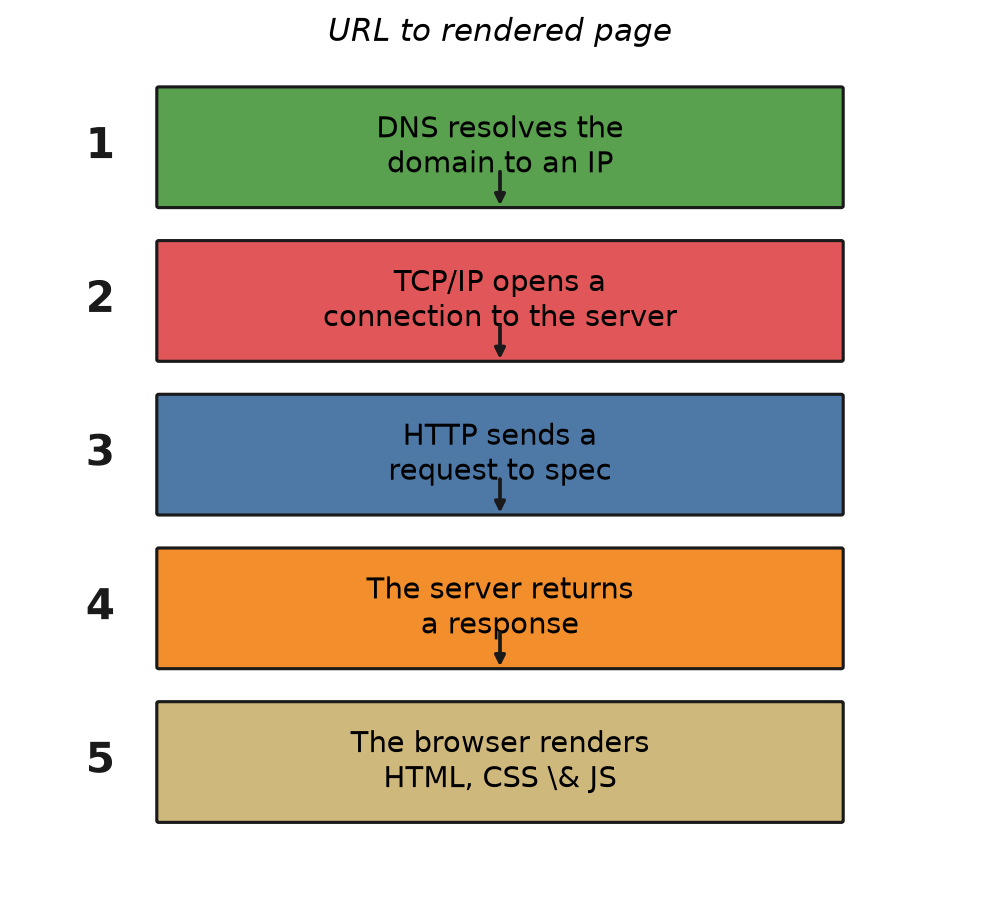
\includegraphics[width=\textwidth]{img/request_lifecycle.png}\\
            {\scriptsize URL to rendered page, one layer at a time.}
        \end{column}
    \end{columns}
    \bottomcite{Textbook Ch.~5, ``What Happens When You Load a Web Page?''}
\end{frame}

\begin{frame}{The lower stack: client--server, TCP/IP \& DNS}
    \begin{columns}[T]
        \begin{column}{0.6\textwidth}
            Every scrape and API call is one \textbf{request--response} cycle: a \textbf{client} (your browser, your Python script) asks a \textbf{server} for a resource.

            \vspace{0.8em}

            \textbf{TCP/IP --- the transport.} Every machine on a public network has an IP address. IPv4 offers $2^{32}\approx4.3$ billion of them; IPv6 offers $2^{128}\approx3.4\times10^{38}$. Data hops router to router to arrive.

            \vspace{0.8em}

            \textbf{DNS --- the address book.} It maps a name like \texttt{en.wikipedia.org} to an IP. Names are hierarchical --- \texttt{subdomain.domain.TLD} --- and services follow conventions: \texttt{api.agency.gov}, \texttt{data.agency.gov}.
        \end{column}
        \begin{column}{0.36\textwidth}
            \centering
            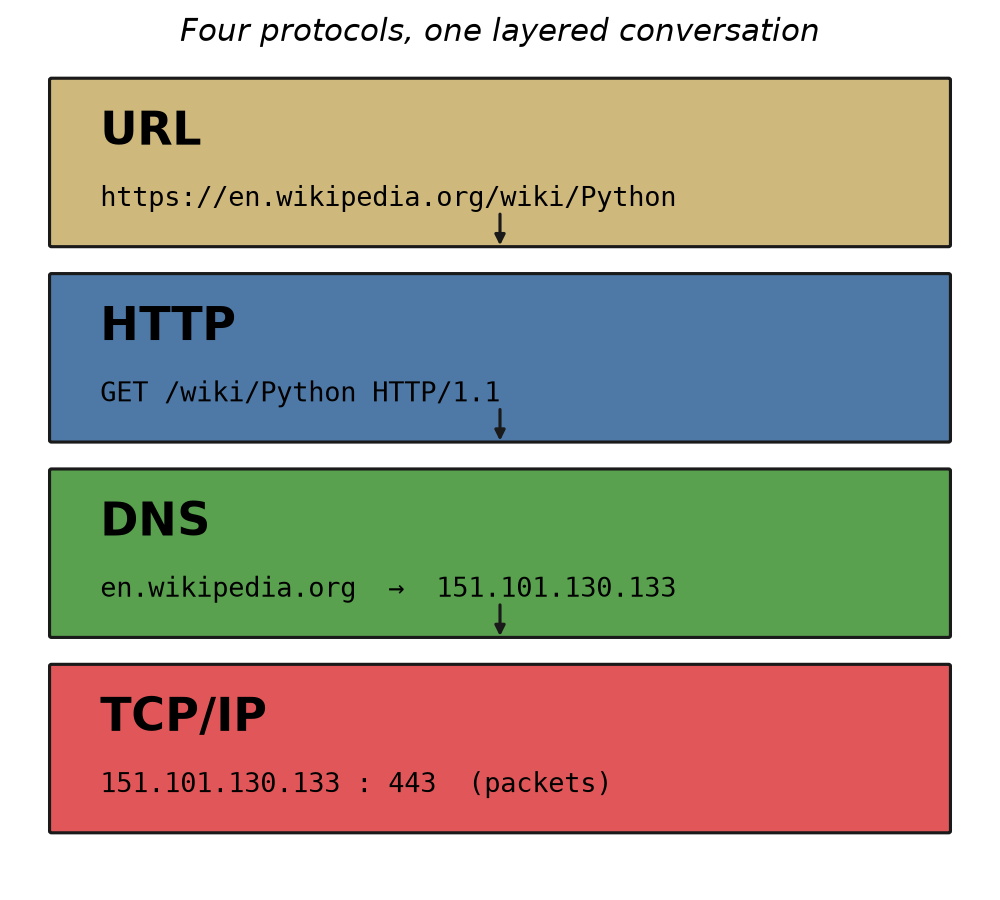
\includegraphics[width=\textwidth]{img/protocol_stack.png}\\
            {\scriptsize Four protocols, one layered conversation.}
        \end{column}
    \end{columns}
    \bottomcite{Textbook Ch.~5, ``The Client--Server Model,'' ``TCP/IP,'' and ``DNS.''}
\end{frame}

\begin{frame}{See it yourself: browser developer tools}
    \begin{columns}[T]
        \begin{column}{0.52\textwidth}
            Before writing a line of code, inspect the page by hand. Open dev tools with \texttt{Ctrl+Shift+I} or \texttt{F12} (\texttt{Cmd+Opt+I} on a Mac).

            \vspace{0.8em}

            \textbf{Inspector} shows the HTML as a tree you can hover and expand. Start on a simple Wikipedia article --- commercial sites bury structure under tracking scripts.

            \vspace{0.8em}

            \textbf{Network} reveals every request a page makes --- often hundreds: HTML, CSS, JS, images, fonts, trackers. Each shows a URL, method, status code, and headers like \texttt{User-Agent} and \texttt{Cookie}.
        \end{column}
        \begin{column}{0.44\textwidth}
            \centering
            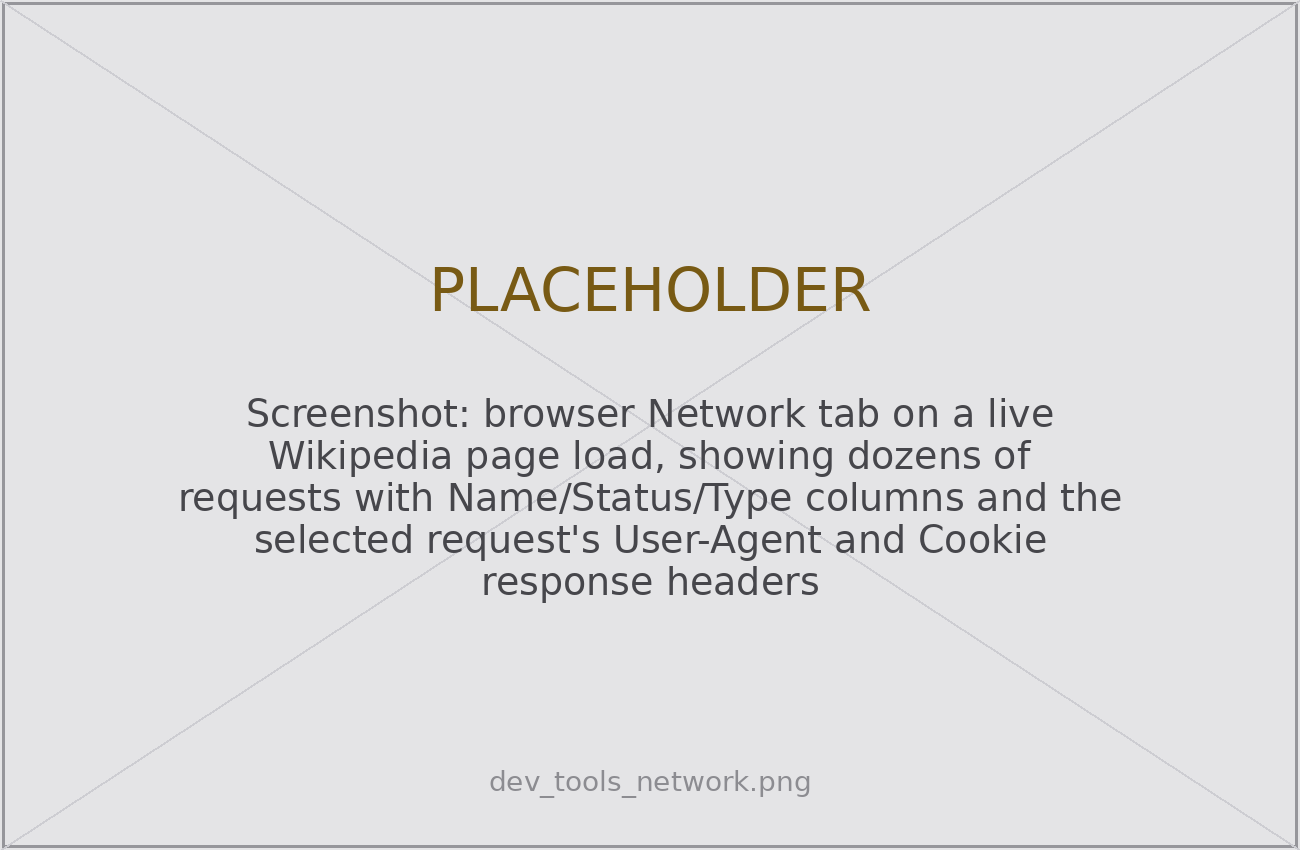
\includegraphics[width=\textwidth]{img/dev_tools_network.png}\\
            {\scriptsize The Network tab: one page load, dozens of requests.}
        \end{column}
    \end{columns}
    \bottomcite{Textbook Ch.~5, ``Browser Developer Tools.''}
\end{frame}

\begin{frame}{The upper stack: HTTP status codes \& URLs}
    \begin{columns}[T]
        \begin{column}{0.54\textwidth}
            \textbf{HTTP} structures the conversation: a request carries a method (GET, POST, \dots) and headers; a response carries a \textbf{status code}:
            \begin{itemize}\small
                \item \textcolor{tab-green}{\textbf{200}} OK --- the body has your data
                \item \textcolor{tab-blue}{\textbf{301/302}} redirect --- follow \texttt{Location}
                \item \textcolor{tab-red}{\textbf{403}} forbidden --- often a missing \texttt{User-Agent}
                \item \textcolor{tab-orange}{\textbf{404}} not found \quad \textcolor{tab-red}{\textbf{429}} slow down
                \item \textcolor{tab-purple}{\textbf{500}} the server's problem, not yours
            \end{itemize}
        \end{column}
        \begin{column}{0.42\textwidth}
            \textbf{URLs} identify the target, with a fixed structure:

            \vspace{0.6em}

            \centering
            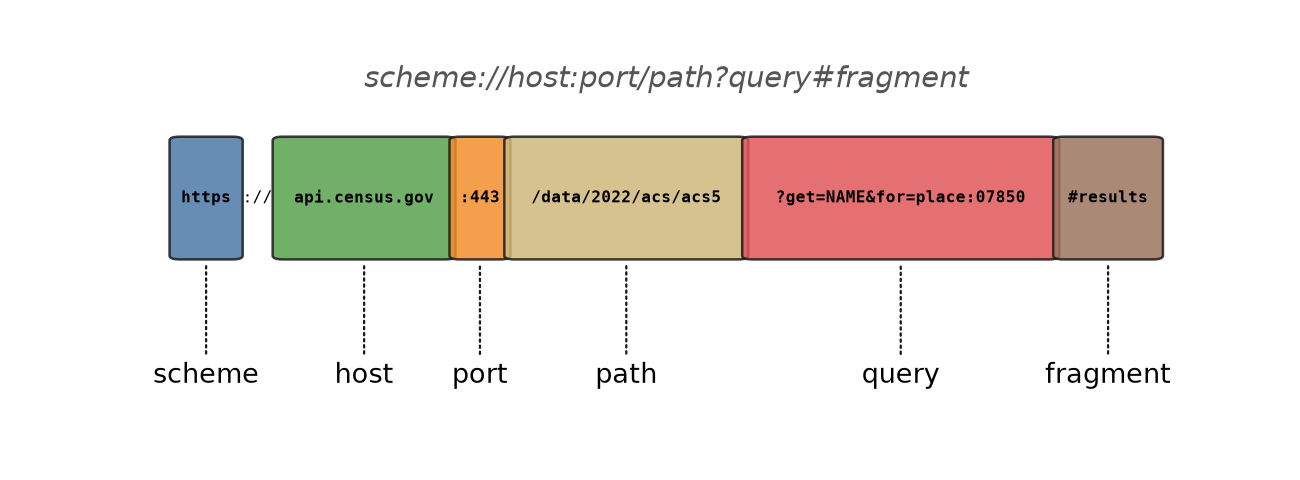
\includegraphics[width=\textwidth]{img/url_anatomy.png}\\
            {\scriptsize \texttt{scheme://host:port/path?query\#fragment}}
        \end{column}
    \end{columns}
    \bottomcite{Textbook Ch.~5, ``HTTP: The Application Layer'' \& ``URLs: Anatomy and Parsing.''}
\end{frame}

\begin{frame}{What the notebook covers}
    This week's companion notebook walks \emph{down} the stack, then back \emph{up}:
    \begin{itemize}
        \item \textbf{Addressing} --- find your local and public IP (\texttt{socket}, \texttt{ipify}); resolve a domain with \texttt{dns.resolver}; trace the route to Wikipedia
        \item \textbf{Diagnosis} --- a \texttt{diagnose\_request()} helper that reads status codes, headers, and redirect history
        \item \textbf{A live API} --- the Wikimedia pageviews endpoint: fix a 403, parse the JSON, and plot a time series
        \item \textbf{Scaling up} --- a \texttt{Session} with retries; parsing \emph{and} building URLs with \texttt{urllib.parse}
    \end{itemize}

    \vspace{0.6em}

    \begin{alertblock}{Connecting to Ch.~2 (Ethics) \& Ch.~3 (Post-API)}
        ``View source'' and network inspection exist because the web was built as \textbf{open} public infrastructure --- open standards in public RFCs, not proprietary products. That same openness is what platforms increasingly fight, the tension you will study in the post-API age.
    \end{alertblock}
\end{frame}

% =========================================================================
\section{Wednesday · Notebook Lab}
% =========================================================================

\begin{frame}[fragile]{Where am I? Where is the server?}
    Your public IP is how the internet sees you; DNS is how a name becomes a routable address:
\begin{lstlisting}
import requests
import dns.resolver

# Your public IP, as servers on the internet see it
print(requests.get("https://api.ipify.org?format=json").json())
# {'ip': '128.138.xxx.xxx'}

# Resolve a domain name to its IP address(es)
for rec in dns.resolver.resolve("en.wikipedia.org", "A"):
    print("IP address:", rec)
\end{lstlisting}
    \begin{alertblock}{\texttt{scapy} traceroute needs root}
        \footnotesize The notebook's \texttt{traceroute("en.wikipedia.org")} maps each router hop, but raw packets require admin privileges (Npcap on Windows). Can't run it? Read along --- nothing later depends on it.
    \end{alertblock}
    \bottomcite{Textbook Ch.~5, ``TCP/IP'' \& ``DNS.'' \texttt{socket.gethostbyname} often returns a loopback address --- query an external service for your real public IP.}
\end{frame}

\begin{frame}[fragile]{Diagnosing HTTP errors, not guessing}
    The status code says \emph{what} failed; the full response says \emph{why}. Read both:
\begin{lstlisting}
def diagnose_request(url, headers=None):
    try:
        r = requests.get(url, headers=headers, timeout=10)
    except requests.exceptions.ConnectionError:
        return print("Connection failed:", url)
    print("Status:", r.status_code)
    print("Content-Type:", r.headers.get("Content-Type", "n/a"))
    print("Bytes:", len(r.content))
    if r.history:                       # a redirect chain
        print("Redirected from:", r.history[0].url)
    return r
\end{lstlisting}
    A \textbf{403} from an API usually means a missing \texttt{User-Agent} (a one-line fix); a \textbf{403} from a news site may block scraping outright. A \textbf{429} means slow down; a \textbf{500} is the server's problem --- retry later.
    \bottomcite{Textbook Ch.~5, ``Diagnosing HTTP Errors.''}
\end{frame}

\begin{frame}[fragile]{Make an API call, get a time series}
    \begin{columns}[T]
        \begin{column}{0.56\textwidth}
        The Wikimedia pageviews API rejects the default client with \textbf{403} --- add a meaningful \texttt{User-Agent} and it returns \textbf{200}:
\begin{lstlisting}
url = ("https://wikimedia.org/api/rest_v1/"
       "metrics/pageviews/per-article/en.wikipedia/"
       "all-access/all-agents/"
       "University_of_Colorado_Boulder/daily/"
       "20240101/20240131")
ua = {"User-Agent": "WebDataScience/1.0 (you@colorado.edu)"}
data = requests.get(url, headers=ua).json()
\end{lstlisting}
        Reshape the nested JSON, then plot it:
\begin{lstlisting}
df = pd.DataFrame(data["items"])
df["timestamp"] = pd.to_datetime(df["timestamp"],
                                 format="%Y%m%d00")
df.plot(x="timestamp", y="views")
\end{lstlisting}
        \end{column}
        \begin{column}{0.4\textwidth}
            \centering
            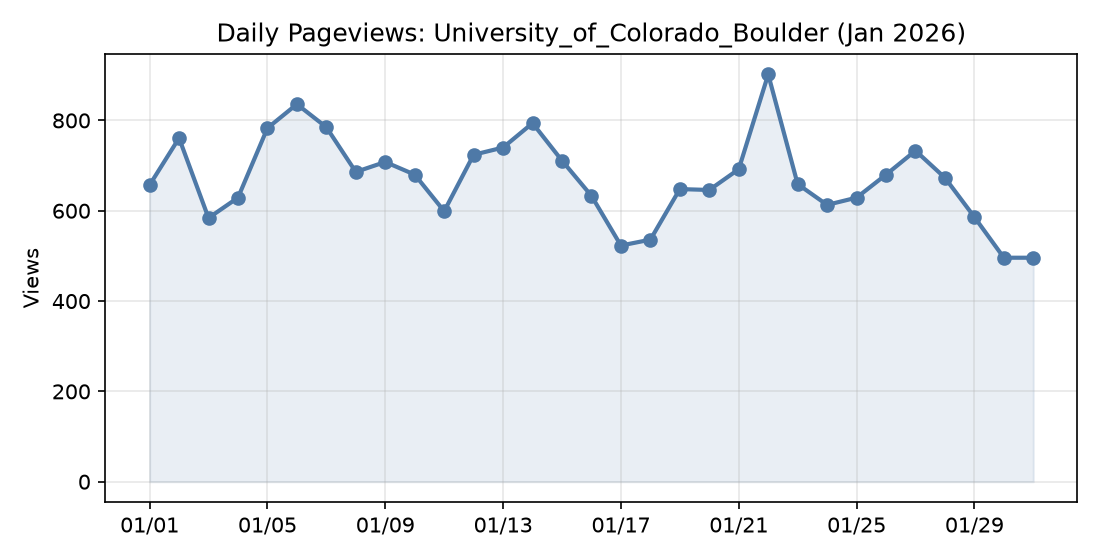
\includegraphics[width=\textwidth]{img/pageviews_timeseries.png}\\
            {\scriptsize Daily pageviews --- spikes line up with real-world events.}
        \end{column}
    \end{columns}
    \bottomcite{Textbook Ch.~5, ``Making API Requests with Custom Headers.''}
\end{frame}

\begin{frame}[fragile]{A loop over one host is your cue for a Session}
    A bare \texttt{requests.get()} opens a fresh connection every time. Looping over many URLs at one host? Create a \texttt{Session} --- it reuses the connection, remembers headers, and retries automatically:
\begin{lstlisting}
from requests.adapters import HTTPAdapter
from urllib3.util.retry import Retry

session = requests.Session()
session.headers.update({"User-Agent": "WebDataScience/1.0 (you@colorado.edu)"})

# Retry 429/5xx with backoff of 1s, 2s, 4s; honors Retry-After
retries = Retry(total=3, backoff_factor=1,
                status_forcelist=[429, 500, 502, 503, 504])
session.mount("https://", HTTPAdapter(max_retries=retries))

for article in ["Web_scraping", "Data_science"]:
    r = session.get(f"https://en.wikipedia.org/wiki/{article}")
\end{lstlisting}
    Six lines of setup replace the hand-rolled backoff loop --- and carry over unchanged into the scraping, Wikipedia, and government-data chapters.
    \bottomcite{Textbook Ch.~5, ``Connections, Sessions, and Retries.''}
\end{frame}

\begin{frame}[fragile]{Parse --- and build --- URLs with the right tool}
    Never parse a URL with a regular expression. \texttt{urllib.parse} follows the spec:
\begin{lstlisting}
from urllib.parse import urlparse, parse_qs, quote

u = urlparse("https://api.census.gov/data/2022/acs/acs5?get=NAME&for=place:07850")
u.scheme, u.netloc, u.path   # 'https', 'api.census.gov', '/data/2022/acs/acs5'
parse_qs(u.query)            # {'get': ['NAME'], 'for': ['place:07850']}
\end{lstlisting}
    Two API styles need two builders. \textbf{Path-segment} APIs need \texttt{quote()} on each component; \textbf{query-parameter} APIs take a \texttt{params=} dict and let \texttt{requests} do the escaping:
\begin{lstlisting}
quote("AC/DC", safe="")   # 'AC%2FDC' -- the slash MUST be encoded
requests.get(base, params={"titles": "University of Colorado Boulder"})
\end{lstlisting}
    Mixing them up --- query-encoding a value the API expects in its path --- is a classic source of confusing 404s.
    \bottomcite{Textbook Ch.~5, ``URLs: Anatomy and Parsing'' \& ``Building URLs Programmatically.''}
\end{frame}

\begin{frame}{Lab: work these, then show-and-tell}
    \begin{columns}[T]
        \begin{column}{0.62\textwidth}
            Work through the chapter's exercises in pairs:
            \begin{enumerate}\small
                \item Network tab: a Wikipedia article vs.\ a news site --- how many requests? What fraction is content vs.\ tracking?
                \item Resolve five related domains with \texttt{dns.resolver} --- do any share an IP address?
                \item Plot pageviews for three related articles; hypothesize what caused the spikes
                \item Write \texttt{diagnose\_url()} and test it on a 200, a 404, a redirect, an API, and a blocked site
                \item \textcolor{tab-purple}{\textbf{5617:}} profile a site's delivery infrastructure --- redirect chain, CDN headers, traceroute hops --- in a 500-word memo
            \end{enumerate}
        \end{column}
        \begin{column}{0.34\textwidth}
            \begin{block}{Show-and-Tell}
                \footnotesize Come ready to share:
                \begin{itemize}\footnotesize
                    \item a challenging bug
                    \item interesting data you pulled
                    \item a provocation for a research design
                \end{itemize}
            \end{block}
        \end{column}
    \end{columns}
\end{frame}

\begin{frame}[standout]
    When a request fails, don't guess.\\
    Ask the stack, in order:\\[0.8em]
    {\large Can I reach the server?\\
    Am I resolving the right address?\\
    What status code came back?\\
    Are my headers correct?\\
    Is my URL well-formed?}
\end{frame}

% =========================================================================
\section{Friday · Textbook Revisions}
% =========================================================================

\begin{frame}{Improving Chapter 5 together}
    \begin{columns}[T]
        \begin{column}{0.6\textwidth}
            Today we make the book better. Each of you opens a \textbf{pull request} against \texttt{ch-05-protocols.qmd} and reviews a classmate's.

            \vspace{1em}

            The workflow (from Week 1):
            \begin{enumerate}\small
                \item Branch / fork the book repo
                \item Edit the chapter; commit with a clear message
                \item Open a PR describing \textit{what} and \textit{why}
                \item Review two peers' PRs: kind, specific, actionable
            \end{enumerate}
        \end{column}
        \begin{column}{0.36\textwidth}
            \centering
            
\includegraphics[width=\textwidth]{img/pr_review.png}
        \end{column}
    \end{columns}
    \bottomcite{Contributions \& reviews count toward the Textbook Revisions grade (30\%).}
\end{frame}

\begin{frame}{A revision menu for Chapter 5}
    High-value targets --- pick one and scope it to a single PR:
    \begin{itemize}
        \item \textbf{Test the code against live services.} \texttt{api.ipify.org}, \texttt{ip-api.com} (45 req/min), the Wikimedia pageviews API, and DNS results all drift. Run the notebook, report what broke, and fix it.
        \item \textbf{Deepen ``Common Issues to Debug.''} Add a worked \texttt{Retry-After} example, an IPv6 \texttt{AAAA} lookup, or a step-by-step \texttt{scapy}/Npcap install note --- the chapter's thinnest section.
        \item \textbf{Add a figure.} A clean layered-stack diagram, an annotated Network-tab screenshot, or a labeled URL-anatomy figure would anchor the concepts.
        \item \textbf{Strengthen an exercise.} Give the \texttt{diagnose\_url()} exercise expected output, a rubric, or a starter cell so it is self-checking.
        \item \textbf{Extend ``Further Reading.''} Tie the HTTP/1.1 RFC or MDN's HTTP overview to the ``openness'' callout on the web as public infrastructure.
    \end{itemize}
    \bottomcite{Targets drawn from the chapter's callouts, ``Common Issues to Debug,'' and ``Further Reading.''}
\end{frame}

\begin{frame}{What makes a good revision \& a good review}
    \begin{columns}[T]
        \begin{column}{0.48\textwidth}
            \begin{block}{A strong PR}
                \begin{itemize}\small
                    \item One focused change, clearly titled
                    \item Explains the problem it fixes
                    \item Builds (\texttt{quarto render}) without errors
                    \item Matches the book's voice and notation
                    \item Discloses any AI assistance
                \end{itemize}
            \end{block}
        \end{column}
        \begin{column}{0.48\textwidth}
            \begin{block}{A strong review}
                \begin{itemize}\small
                    \item Runs / reads the change, not just skims
                    \item Names specifics (line, claim, code)
                    \item Separates ``must fix'' from ``nice to have''
                    \item Is generous --- assume good faith
                    \item Ends with a clear verdict
                \end{itemize}
            \end{block}
        \end{column}
    \end{columns}
    \vspace{0.5em}
    \centering\small Next week: \textbf{Parsing static web pages} --- turning messy HTML into a clean DataFrame.
\end{frame}

% =========================================================================
\begin{frame}{Key takeaways}
    \begin{enumerate}
        \item The web is a \textbf{layered stack}: TCP/IP transports, DNS resolves names, HTTP structures the conversation, URLs identify the target.
        \item Debugging is \textbf{systematic diagnosis}, not guesswork: reach the server? right address? which status code? headers correct? URL well-formed?
        \item A meaningful \texttt{User-Agent} fixes most \textbf{403}s; backoff or a \texttt{Retry} policy handles \textbf{429}s.
        \item A \texttt{for} loop over one host is your cue to use a \texttt{Session} --- persistent connection, shared headers, automatic retries.
        \item \textbf{Never regex a URL.} \texttt{urllib.parse} both parses and builds; know path-segment (\texttt{quote}) from query-parameter (\texttt{params=}) APIs.
    \end{enumerate}
    \vspace{1em}
    \bottomcite{Reading: Textbook Ch.~5. Related: \textcite{mitchell2018web}; \textcite{vandenbroucke2018practical}; \textcite{mozilladevelopernetwork_HTTP_2023}.}
\end{frame}

\end{document}
